\documentclass[16pt]{article}

\usepackage[a4paper,margin=2cm]{geometry}
\usepackage{amsmath}
\usepackage{mathtools}
\usepackage{tikz}
\usepackage{pgf-pie}
\usepackage{tikz-cd}
\usepackage{cancel}
\usepackage{setspace}
\usepackage[fontsize=16pt]{fontsize}
\usepackage{indentfirst}
\usepackage{afterpage}
\usepackage{caption}

\author{}
\date{}
\title{Fractions\\
\vspace{28pt}
\begin{normalsize}Applied Scholastics, Ferndale WA \end{normalsize}}

\begin{document}

\maketitle
\pagebreak
\tableofcontents
\pagebreak

\begin{spacing}{1.25}

\section{What is a fraction}

In English, a fraction means a small bit of something. You could say “I only took a fraction of your drink.”\\

In arithmetic, a fraction means  equal parts of a whole.\\

It is written as two numbers on top of each other with a line between them, called the fraction bar.\\

\begin{tikzpicture}
  \pie[
    color={white, white},
    hide number,
    radius=2,
    scale font={\fontsize{20}{24}\selectfont},
  ]{50/{$\frac{1}{2}$}, 50/{$\frac{1}{2}$}}

\pie[
    color={white, white, white, white},
    hide number,
    radius=2,
    pos={6,0},
    scale font={\fontsize{20}{24}\selectfont}
    ]{25/$\frac{1}{4}$, 25/$\frac{1}{4}$, 25/$\frac{1}{4}$, 25/$\frac{1}{4}$}
  \pie[
    rotate=180,
    color={white, white},
    pos={12,0},
    explode={0.3, 0},
    radius=2,
    before number=\phantom,
    after number=,
    sum=auto
    ]{25/{\fontsize{20}{24}\selectfont $\frac{1}{4}$}, 75/{\fontsize{20}{24}\selectfont $\frac{3}{4}$}}
\end{tikzpicture}\\

There are some special words used to name some fractions. A half means a piece of something that has been cut into 2 pieces. A third means a piece of something that has been cut into 3 pieces. For fractions of things that have been cut into 4 or more pieces, the word ending -th or -eth is added to the number to name that fraction. A piece of something that was cut into 20 pieces would be called a twentieth. That gets shortened usually to a $20^{\textrm{th}}$, or written $\frac{1}{20}$ as a fraction.\\

\pagebreak

\subsection*{Denominator}
In English, denominator means something that tells you what group or type of thing something belongs to. It gives something a name. 
Doing a lot of sports is the denominator that names someone as a sporty person.

In maths, the denominator is the total number of parts that the whole has been broken up into. It names what kind of fraction it is. A denominator of 2 names the fraction as halves.

In maths, the denominator is the total number of parts that the whole has been broken up into. It tells you what kind of fraction it is.

\subsection*{Numerator}
The number above the fraction bar is called the numerator. It means the number of parts that are being talked about.

$\frac{1}{2}$ means that something is in two parts and that we are talking about one of those parts. $\frac{3}{4}$ means something is in 4 parts and that we have 3 of them.

\vspace{28pt}
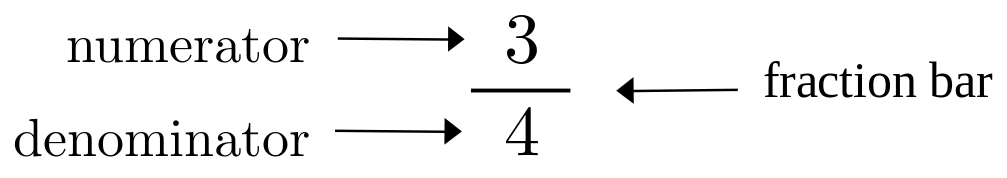
\includegraphics[width=0.7\textwidth]{fraction diagram.png}
\vspace{14pt}
\begin{center}
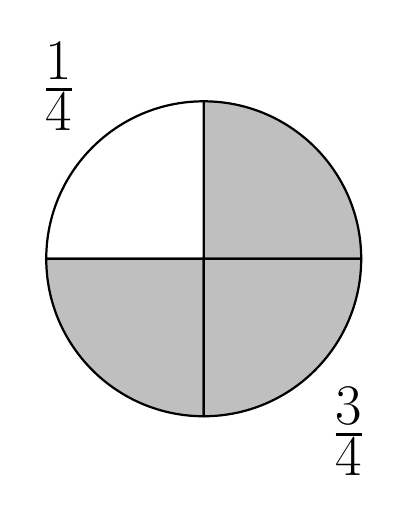
\begin{tikzpicture}
  \pie[
    color={lightgray, white, lightgray, lightgray},
    radius=2,
    before number=\phantom,
    after number=,
    sum=auto
    ]{25/{}, 25/{\fontsize{30}{34}\selectfont $\frac{1}{4}$}, 25/{}, 25/{\fontsize{30}{34}\selectfont $\frac{3}{4}$}}
\end{tikzpicture}
\end{center}

\pagebreak

\section{Equivalent fractions}

\subsection*{Equivalent}
Equivalent means the same as or just as good as. Coke and Pepsi are equivalent drinks. They taste the nearly same so it doesn’t matter which one you get.

In maths, things are equivalent if they are different ways of writing the same amount. $3+3$ is equivalent to $2 \times 3$.\\

\subsection*{Express} When you have an idea it starts in your mind. For someone else to know what that idea is, you have to put the idea into the real world so that it can be heard or seen. Talking and writing are ways of expressing ideas to others. There are many ways to exress ideas.

In maths, express means to put a maths idea into maths symbols that others can read. $3 \times 4 + 2$ is an idea expressed in maths. Its like using words in a sentence but you are using the numbers and symbols of maths.

\pagebreak

\subsection*{Equivalent fractions}
Equivalent fractions are where you express the same amount in different ways. One half, $\frac{1}{2}$, two quarters, $\frac{2}{4}$, and four eighths, $\frac{4}{8}$ all express the same amount even though they have different numerators and denominators. They are called equivalent fractions.\\

\begin{tikzpicture}
  \pie[
    color={lightgray, white},
    hide number,
    radius=2,
    scale font={\fontsize{20}{24}\selectfont},
  ]{50/{$\frac{1}{2}$}, 50/{$\frac{1}{2}$}}

\pie[
    color={lightgray, lightgray, white, white},
    hide number,
    radius=2,
    pos={6,0},
    scale font={\fontsize{20}{24}\selectfont}
    ]{25/$\frac{1}{4}$, 25/$\frac{1}{4}$, 25/$\frac{1}{4}$, 25/$\frac{1}{4}$}

\pie[
    color={lightgray, lightgray, lightgray, lightgray, white, white, white, white},
    hide number,
    radius=2,
    pos={12,0},
    scale font={\fontsize{20}{24}\selectfont}
    ]{12.5/$\frac{1}{8}$, 12.5/$\frac{1}{8}$, 12.5/$\frac{1}{8}$, 12.5/$\frac{1}{8}$, 12.5/$\frac{1}{8}$, 12.5/$\frac{1}{8}$, 12.5/$\frac{1}{8}$, 12.5/$\frac{1}{8}$}

\end{tikzpicture}

\vspace{28pt}
Half of something, $\frac{1}{2}$, is the same amount as two quarters of it, $\frac{2}{4}$, and its also the same as four eighths, $\frac{4}{8}$. They are equivalent fractions.

\pagebreak

\subsection*{Making equivalent fractions}

To make equivalent fractions you multiply or divide both the numerator and denominator by the same number. The amount that the fraction expresses does not change as long as you do the same thing to both the top and the bottom of a fraction.

If you have the fraction $\frac{2}{4}$, you can multiply both the numerator and denominator by 2 to get the equivalent fraction $\frac{4}{8}$. You can divide both the numerator and denominator by 2 to get the equivalent fraction $\frac{1}{2}$.
$$\frac{2}{4} = \frac{2 \times 2}{4 \times 2} = \frac{4}{8}$$
$$\frac{2}{4} = \frac{2 \div 2}{4 \div 2} = \frac{1}{2}$$\\

Think of some fractions and change them into equivalent fractions until you can do it easily and you're sure that you're doing it right every time.

\pagebreak

\section{Simplifying fractions}

\subsection*{Simplify} Simplify means to make something simple so that it's easier. A fraction is easier to work with when it has been simplified. You do that by changing it into an equivalent fraction that has smaller numbers in it. When you simplify $\frac{4}{8}$ it becomes $\frac{1}{2}$.

\subsection*{Greatest} In English, greatest means the best, as in a circus where they say its the Greatest Show on Earth. Greatest also meant biggest, like when you say things like my greatest fear is spiders.

In maths, greatest means the biggest number, like if you compare between 9 and 7, and say that 9 is the greatest.

\subsection*{Common} Common means shared by two or more people or things, like when people share something in common.

In maths common means that two things have the same number in them somewhere. If you had two groups of numbers you would say that the common numbers were the ones that were in both groups. Say 2, 3, 4, 5 and 4, 5, 6, 7. The common numbers there are 4 and 5.

\subsection*{Factor} In English, a factor means a part of something. People might talk about the factors of some situation, meaning the different parts of it, like how much time or money you have.

In maths a factor is a part of multiplication. Most numbers are made up of smaller numbers, called factors, that can be multiplied to give the first number. For example, the factors of 8 are 1, 2, 4 and 8, because 1 $\times$ 8, 2 $\times$ 4, 4 $\times$ 2, and 8 $\times$ 1 all equal 8.

\subsection*{Greatest Common Factor}
The largest number that divides evenly into both the numerator and denominator of a fraction is called the greatest common factor.

You divide the numerator and the denominator by the greatest common factor to get the simplified fraction.

Simplified fractions are easier to work with. Always simplify a fraction if you can, both before you try to add, subtract, multiply or divide them, and in writing your final answer.

\subsubsection*{Cancelling}
To cancel something means to cross it out. To cancel a fraction means to divide the numerator and the denominator by their greatest common factor and cross them out and replace them.

For example, for $\frac{4}{8}$, the largest number that divides evenly into both the numerator and denominator is 4, but you don't bother to write that. You just cross out the 4 and write a 1, and cross out the 8 and write a 2. That gives you the equivalent simplified fraction of 1/2.

$$\text{So instead of writing }\frac{4}{8} = \frac{4 \div 4}{8 \div 4} = \frac{1}{2}\text{, you just write }\frac{4}{8} = \frac{^1 \cancel{4}}{\cancel{8}_2}\text{.}$$

\subsection*{Finding the Greatest Common Factor}

\subsubsection*{Knowing the times table} You can often just simplify fractions in your head, if you know the times table well. With practice you can get good enough that you will know the greatest common factor right away without having to think much about it.
For example, maybe you can see that the greatest common factor needed to simplify $\frac{3}{9}$ is 3.
$$\frac{3}{9} = \frac{3 \div 3}{9 \div 3} = \frac{1}{3} \text{   or by cancelling you write }\frac{^1\cancel{3}}{\cancel{9}_3} = \frac{1}{3}$$

\subsubsection*{Using any factor} If you can't find greatest common factor, it will still work if you find just any common factor and use that to start with. You will get a simpler fraction and then you can look at that one for a new common factor. Keep going until you are sure there are no more common factors.\\

Say you have to simplify $\frac{63}{84}$, and you spot that 3 divides evenly into both 63 and 84. You cancel both numbers and replace them.

$$\frac{^{21}\cancel{63}}{\cancel{84}_{28}}$$

Now you have $\frac{21}{28}$ and you see that 21 and 28 are multiples of 7, so you cancel both numbers again and replace them.

$$\frac{63}{84} = \frac{^{21}\cancel{63}}{\cancel{84}_{28}} = \frac{^3\cancel{21}}{\cancel{28}_4} = \frac{3}{4}$$

\pagebreak

\subsubsection*{Listing out all the factors}
You can also work out the factors and write them down to pick the greatest common factor. You’ll definitely get a right answer that way.

\vspace{28pt}
For example, to simplify $\frac{63}{105}$,

\vspace{28pt}
factors of 63: 1, 3, \textcircled{7,} 9, 21, 63

factors of 105: 1, 3, 5, \textcircled{7,} 15, 21, 35, 105

\vspace{28pt}
The greatest common factor of 63 and 105 is 7.

$$63 = \div 7 = 9 \text{ and }105 \div 7 = 15\text{, so }\frac{63}{105} = \frac{9}{15}$$

$$\text{You would write it as }\frac{^9 \cancel{63}}{\cancel{105}_{15}}$$

\vspace{28pt}
Pick some fractions and practice finding greatest common factors and simplifying until you can do it easily and get it right every time.

\pagebreak

\subsection*{Using Prime Factors to Simplify Fractions}
A foolproof way to simplify fractions is to find the prime factors of the numerator and denominator and rewrite the fraction as their product. Doing that can be easier than finding the greatest common factor when the numbers in the fraction get too big.

Remember prime factor trees? Product means the answer you get from multiplying. The product of 2 and 3 is 6, for example. Any number that isn't a prime number can be expressed as a product of its prime factors.

\begin{figure}[ht]
  \centering
  \begin{minipage}{0.4\textwidth}
    \centering
    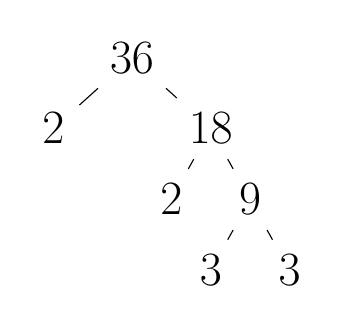
\begin{tikzpicture}[level distance=0.9cm,
      level 1/.style={sibling distance=2cm},
      level 2/.style={sibling distance=1cm}]
      \node {36}
        child {node {2}}
        child {node {18}
          child {node{2}}
          child {node {9}
            child {node {3}}
            child {node {3}}}
        };
    \end{tikzpicture}
\caption*{\hspace{1cm}$36 = 2 \times 2 \times 3 \times 3$}
    \label{fig:tree36}
  \end{minipage}%
  \hfill
  \begin{minipage}{0.4\textwidth}
    \centering
    \begin{tikzpicture}[level distance=0.9cm,
      level 1/.style={sibling distance=2cm},
      level 2/.style={sibling distance=1cm}]
      \node {48}
        child {node {2}}
        child {node {24}
          child {node{2}}
          child {node {12}
            child {node {2}}
            child {node {6}
              child {node {2}}
              child {node {3}}}
        }};
    \end{tikzpicture}
    \caption*{\hspace{1cm}$48 = 2 \times 2 \times2 \times 2 \times 3$}
    \label{fig:tree48}
  \end{minipage}
\end{figure}

$$\frac{36}{48} &= \frac{2 \times 2 \times 3 \times 3}{2 \times 2 \times2 \times 2 \times \times 3}$$\\

Now it's easy to see what to cancel.

$$\frac{36}{48} = \frac{{^1\cancel{2 \times 2}} \times 3 \times ^1{\cancel{3}}}{^1{\cancel{2 \times 2}} \times2 \times 2 \times \times {\cancel{3}}_1} = \frac{1 \times 3 \times 1}{1 \times 2 \times 2 \times 1} = \frac{3}{4}$$\\

Practice doing this until you can do it easily and get right answers.

\pagebreak

\section{Proper fractions \\and Improper fractions}

\subsection*{Proper} In English, proper mean that something is done right. Having proper manners means that you are doing the right thing.

Fraction means equal parts of a whole thing. It means less than 1 of something and not the whole thing. A fraction is proper when the numerator is smaller than the denominator, meaning that the fraction is less than 1. $\frac{3}{4}$ is a proper fraction.

\subsection*{Improper} Improper means that something is not being done right. Improper behaviour means bad conduct or being rude.

An improper fraction is one where the numerator is bigger than the denominator, so that the value of the fraction is greater than 1. It's not just an equal part of something so it's not properly a fraction. It's some value expressed as a fraction but it's not really a fraction, so it's called an improper fraction.

For example, $\frac{3}{2}$ means that you have 3 halves of something, an improper fraction, just like $\frac{13}{7}$ is also an improper fraction.

\pagebreak

\subsection*{Changing a whole number \\ into an improper fraction}
Sometimes you have to express a whole number as a fraction. That’s done by using the whole number as the numerator and using a denominator of 1.

Fractions and dividing are similar things. $\frac{1}{2}$ is just another way of expressing $1 \div 2$. Any number divided by 1 doesn't change the number, so a fraction with a denominator of 1 has the same value as just its numerator.\\

For example, $236 = 236 \div 1 = \frac{236}{1}$.\\

You can change any whole number into an improper fraction just by writing it as a fraction over 1.\\

Pick some whole numbers and practice changing them into improper fractions until you can do it easily.

\pagebreak

\section{Mixed fractions}

Mixed means that two or more things have been put together. You might hear of a dog being a mixed breed. A labradoodle is a mix of labrador and poodle.

A fraction that is a mix of a whole number plus a proper fraction is called a mixed fraction.

$1\frac{3}{4}$ is really saying $1 + \frac{3}{4}$, so it is a mixed fraction.

As well as simplifying a fraction if you can, you also change an improper fraction to a mixed fraction when you are writing your final answer.

\subsection*{Changing an improper fraction \\into a mixed fraction}
An improper fraction is greater than 1, so it's really a whole number plus a proper fraction.

To change an improper fraction to a mixed fraction you divide the numerator by the denominator. The result is the whole number part and the remainder is the numerator of the fraction part.\\

For example, $\frac{22}{7}$:

22 $\div$ 7 = 3, with a remainder of 1.

So $\frac{22}{7}$ = $3 \frac{1}{7}$.\\

Practice changing improper fractions into mixed fractions until you can do it easily and you know you are doing it right.

\pagebreak

\subsection*{Changing a mixed fraction \\ into an improper fraction}
Sometimes you have to change a mixed fraction back into an improper fraction. To do that you split the mixed fraction into the whole number part and the fraction part. Then you change the whole number part into an improper fraction and add the two fractions.

To find the numerator of the whole number part, multiply the whole number and the denominator of the fraction part.

The denominator of the whole number part is the same denominator as the fraction part.

\begin{doublespace}
For example, $2 \frac{3}{5}$ :

$2 \frac{3}{5} = 2 + \frac{3}{5}$

2 (whole number part) $\times$ 5 (denominator of fraction part) = 10,

so 2 (as a whole number) = $\frac{{2 \times 5}}{5} = \frac{10}{5}$ (as an improper fraction)

and $2 \frac{3}{5}$ (mixed fraction) = $\frac{10}{5}$ + $\frac{3}{5} = \frac{13}{5}$ (improper fraction.)
\end{doublespace}

\vspace{28pt}
Practice changing mixed fractions into improper fractions until you can do it easily.

\pagebreak

\section{Multiplying fractions}
Multiplying two fractions is easy. You just multiply the two numerators and the two denominators and that’s your answer.

For example, $\frac{3}{7} \times \frac{5}{9} = \frac{15}{63}$.

And then simplify your answer, of course. $\frac{^5\cancel{15}}{\cancel{63}_{21}} = \frac{5}{21}$.\\

In word problems, the word "of" means "times" Things such as "seven eighths of fifteen" are solved by doing $\frac{7}{8}\times15=\frac{105}{8}=13\frac{1}{8}$.\\

Practice multiplying fractions until you can do it easily.

\subsection*{Simplifying before Multiplying}
It is easier to simplify fractions before multiplying because the numbers will be smaller, and the answer will already be simplified.

$$\frac{9}{15} \times \frac{3}{9} =
\frac{{^3\cancel{9}}}{{\cancel{15}_5}} \times \frac{{^1\cancel{3}}}{{\cancel{9}_3}} = \frac{1}{3}$$

\subsubsection*{Cross-Cancelling}
Because the order doesn't matter when you multiply, you can cancel either denominator with either numerator.

$$\frac{3}{10} \times \frac{2}{5} = \frac{{3 \times 2}}{{10 \times 5}} = \frac{{2 \times 3}}{{10 \times 5}} = \frac{2}{10} \times \frac{3}{5}$$

$$\text{That's why you can do }\frac{3}{{\cancel{10}_5}} \times \frac{{^1\cancel{2}}}{5} = \frac{3}{5} \times \frac{1}{5} = \frac{3}{25}\text{.}$$

You can also do this with any number of fractions.

$$\frac{4}{5} \times \frac{3}{4} \times \frac{2}{3} = \frac{{^1\cancel{4}}}{5} \times \frac{{^1\cancel{3}}}{{\cancel{4}_1}} \times \frac{2}{{\cancel{3}_1}} = \frac{1 \times 1 \times2}{5 \times 1 \times 1} = \frac{2}{5}$$

\subsubsection*{Multiplication by Switching Numerators}
Instead of cross cancelling it is also possible to reverse the order of multiplication in the numerators resulting in easily simplifies fractions.
\begin{align*}
\frac{21}{5} \times \frac{15}{14}
 = \frac{(21 \times 15)}{(5 \times 14)}
&= \frac{(15 \times 21)}{(5 \times 14)}\\
&= \frac{15}{5} \times \frac{21}{14}\\
&= \frac{3}{1} \times \frac{3}{2} = \frac{9}{2}
\end{align*}

\subsection*{Multiplying mixed fractions}
To multiply mixed fractions, convert any mixed fraction to an improper fraction before you do the multiplication.\\
For example, $1 \frac{1}{3} \times 2 \frac{1}{4}$

First, convert both fractions to improper fractions.

$$1 \frac{1}{3} = \frac{3}{3} + \frac{1}{3} = \frac{4}{3} \text{ and } 2 \frac{1}{4} = \frac{8}{4} + \frac{1}{4} = \frac{9}{4}$$

Then you can multiply $\frac{4}{3} \times \frac{9}{4} = \frac{36}{12}$

Then simplify by finding the greatest common factor of 36 and 12:

factors of 36:	1, 2, 3, 4, $\textcircled{6}$, 18, 36

factors of 12:	1, 2, 3, 4, $\textcircled{6}$, 12.

The greatest common factor of 36 and 12 is 6, so

$$\frac{36}{12} = \frac{36 \div 6}{12 \div 6} = \frac{^6 \cancel{36}}{\cancel{12}_2} = \frac{6}{2}$$

Then change $\frac{6}{2}$ back to a proper fraction, $\frac{6}{2} = 6 \div 2 = 3$, with no remainder, and now we have $1 \frac{1}{3} \times 2 \frac{1}{4} = 3$.

\subsubsection*{Multiplying Mixed Fractions\\by Making Them Whole Numbers}
A fraction multiplied by its denominator becomes a whole number, which can simplify multiplications of fractions.\\
$$36 \times 3 \frac{1}{2} = 36 \div 2 \times 3 \frac{1}{2} \times 2 = 18 \times 7 = 126$$

\subsubsection*{Multiplying Mixed Fractions\\by Using Decimal Fractions}

\begin{figure}[ht]
\begin{minipage}[b]{0.5\linewidth} \centering 
36 \times 3 \frac{1}{2} =
\end{minipage}
\begin{minipage}[b]{0.5\linewidth} \centering 
\begin{tabular}{c@{\,}c@{\,}c@{\,}c@{\,}c@{\,}c}
       & &3&6&.&0 \\
\times &_{1}&_{3} &3&.&5 \\
\hline
    &^{1}&1&8&0&0 \\
     + &1&0&8&0&0 \\
\hline
      1&2&6&.&0&0 \\
\hline
\hline
\end{tabular}\\
\end{minipage}\end{figure}
(The decimal point is placed at the total number of fractional digits of the factors being mutliplied.)\\

\vspace{28pt}
Practice multiplying lots of mixed fractions until you can do it easily and you know that you can get it right.

\pagebreak

\section{Dividing fractions}
Dividing fractions is easy. You just have to flip one of the fractions first and then multiply them. Reciprocal means existing on both sides. The flipped version of a fraction is called its reciprocal. 

For example,
$$\frac{3}{7} \div \frac{5}{9} = \frac{3}{7} \times \frac{9}{5} = \frac{27}{35}$$

\begin{enumerate}
  \item Take the fraction you want to divide by and flip it to make its reciprocal. For example, if you have $\frac{3}{4}$ as the second fraction, flip it to get $\frac{4}{3}$.
  
  \item Multiply the top number of the first fraction with the top number of the flipped second fraction, and multiply the bottom number of the first fraction with the bottom number of the flipped second fraction. For example, if the first fraction is $\frac{2}{5}$ and the flipped second fraction is $\frac{4}{3}$, multiply them together to get $\frac{2}{5} \times \frac{4}{3}$.
  
  \item If the top and bottom numbers have any common factors, you can cancel them out to make the fraction simpler. Keep simplifying until you can't do it anymore.
\end{enumerate}

For example, divide $\frac{2}{3}$ by $\frac{5}{6}$ :

$$\frac{2}{3} \div \frac{5}{6} = \frac{2}{3} \times \frac{6}{5} = \frac{12}{15}$$

We can simplify that fraction by dividing both the top and bottom numbers by their greatest common factor, which is 3:

$$\frac{12}{15} = \frac{^4\cancel{12}}{\cancel{15}_5} = \frac{4}{5}$$

\vspace{28pt}
Think of some fractions and practice dividing them by each other until you can do it easily.

\pagebreak

\subsection*{Division by Fractions\\by Converting a Term to 1}

A fraction multiplied by its reciprocal is equal to 1, and that can be used to do divisions by fractions.
\begin{align*}
8 \div \frac{1}{4} &= \frac{8}{1} \div \frac{1}{4}
                    = \frac{8 \times 4}{1 \times 1}
                      \div \frac{1 \times 4}{4 \times 1}\\
                   &= \frac{32}{1} \div \frac{4}{4} = 32
\end{align*}
\begin{align*}
8 \div \frac{1}{2} &= \frac{8}{1} \div \frac{1}{2}
                    = \frac{8 \times 2}{1 \times 1}
                      \div \frac{1 \times 2}{2 \times 1}\\
                   &= \frac{16}{1} \div \frac{2}{2} = 16
\end{align*}

\subsection*{Dividing mixed fractions}
The same as for multiplication, for dividing with mixed fractions it's best to convert any mixed fractions to improper fractions first, do the division, and then convert the answer back to a mixed fraction.

\vspace{28pt}
For example, divide $8 \frac{1}{3}$ by 3 :

First convert both fractions to improper fractions:

$$8\frac{1}{3} = \frac{24}{3} + \frac{1}{3} = \frac{25}{3}$$
\begin{center} and \end{center}
$$3 = \frac{3}{1}$$

Flip one of the fractions because we are dividing them, and multiply.

$$\frac{25}{3} \div \frac{3}{1} = \frac{25}{3} \times \frac{1}{3} = \frac{25}{9}$$

Then convert the answer back to a proper fraction:

$$\frac{25}{9} = 25 \div 9 = 2 \text{, and a remainder of 7}$$
$$\text{so, }\frac{25}{9} = 2\frac{7}{9}$$

\vspace{28pt}
Think of some mixed fractions and practice dividing them by each other until you can do it easily and you know that you are getting right answers.

\pagebreak

\section{Fractions\\with different denominators}
Adding or subtracting two fractions that have different denominators is harder than multiplying or dividing them. You can't just add the numerators or you'll get a wrong answer. Also comparing fractions to see which is the bigger or smaller can’t really be done with fractions that have different denominators. You’d just be guessing. The parts that you are adding or subtracting or comparing all have to be the same size or your answer won’t be right.

To add or subtract or compare two fractions with different denominators, you have to change both fractions into equivalent fractions that both have the same denominator.

Common means shared by both people or things, like when two people have something in common, so finding the denominator that both fractions can be changed into is called finding the common denominator. There are a few different ways of doing it.

When both fractions have been converted into equivalent fractions with a common denominator, then you can add or subtract the numerators and you’ll get a right answer.\\

\begin{tikzpicture}
  \pie[
    color={white, white, white, lightgray, lightgray, lightgray},
    hide number,
    radius=1.5,
    scale font={\fontsize{20}{24}\selectfont},
  ]{16.66/{}, 16.66/{}, 16.66/{}, 16.66/{}, 16.66/{}, 16.66/{$\frac{1}{2}$}}

\pie[
    color={white, white, white, white, lightgray, lightgray},
    hide number,
    radius=1.5,
    pos={6,0},
    scale font={\fontsize{20}{24}\selectfont}
    ]{16.66/{}, 16.66/{}, 16.66/{}, 16.66/{}, 16.66/{}, 16.66/{$\frac{1}{3}$}}

\pie[
    color={white, lightgray, lightgray, lightgray, lightgray, lightgray},
    hide number,
    radius=1.5,
    pos={12,0},
    scale font={\fontsize{20}{24}\selectfont}
    ]{16.66/{}, 16.66/{}, 16.66/{}, 16.66/{}, 16.66/{}, 16.66/{$\frac{5}{6}$}}
\end{tikzpicture}

$$\frac{1}{2} + \frac{1}{3} = \frac{3}{6} + \frac{2}{6} = \frac{5}{6}$$

\pagebreak

\subsection*{Using 1 as a fraction\\to make equivalent fractions}
Fractions and dividing are similar things.

$\frac{3}{4}$ means the same as 3 $\div$ 4.

Also you know that any number divided by itself is equal to 1.

That means that you can express 1 as a fraction by having the numerator and denominator being both the same number. That's the same as dividing a number by itself, which will always equal 1.

$$\frac{3}{3} = \frac{1}{1} = \frac{123}{123} = \frac{12345}{12345} = \frac{17}{17} = 1$$

All of these fractions are just different ways of saying 1. You change a fraction into an equivalent fraction by multiplying the top and bottom numbers by the same amount. The reason that works is that you are really just multiplying the fraction by 1.

$$\frac{3}{4} \times \frac{3}{3} = \frac{9}{12}$$

You can convert a fraction to any equivalent fraction that you need by multiplying it by a 1 that has been expressed as a fraction.

Say you are allowed to have $\frac{1}{4}$ of a pizza but it's already been cut into 12 slices. How many twelfths of the pizza are you allowed to have?

4 goes into 12 3 times, so you multiply $\frac{1}{4}$ by $\frac{3}{3}$ to get $\frac{3}{12}$.

So $\frac{1}{4}$ of a pizza = $\frac{3}{12}$ of a pizza or 3 slices.

\vspace{28pt}
Practice changing fractions into different equivalent fractions this way until you can do it easily.

\pagebreak

\section{Comparing fractions}
Comparing two fractions with different denominators isn’t easy.

Which is bigger: $\frac{2}{3}$ or $\frac{3}{5}$ ? You can only really tell once you have converted them into equivalent fractions with the same denominators.

Once you work out that $\frac{2}{3} = \frac{10}{15}$ and $\frac{3}{5} = \frac{9}{15}$, then you can easily see that the answer is $\frac{2}{3}$.

\subsection*{Cross-multiplying}
A shortcut to comparing fractions, so that you don't have to convert them to equivalent fractions, is cross-multiplying. That means multiplying the numerator of one fraction by the denominator of the other fraction. Then you can compare.

\begin{doublespace}
For example, comparing $\frac{2}{3}$ and $\frac{3}{5}$:

$2 \times 5 = 10$ and $3 \times 3 = 9$,

so $\frac{2}{3}$ is greater than $\frac{3}{5}$.
\end{doublespace}

\vspace{28pt}
Pick some pairs of fractions and practice comparing fractions by cross-multiplying until you can do it easily.

\pagebreak

\section{Adding and Subtracting fractions}
Adding and subtracting two fractions with the same denominator is easy. Add or subtract their numerators and write the result over the denominator.

$$\text{For example, }\frac{1}{4} + \frac{2}{4} = \frac{3}{4}\text{, and }\frac{2}{3} - \frac{1}{3} = \frac{1}{3}$$

\vspace{28pt}
You can't just add or subtract the numerators of fractions that have different denominators though. You'll get a wrong answer.

You can't take pizzas that have been cut into thirds and pizzas that have been cut into quarters and just hand out pieces as if they were all the same size. You have to cut both pizzas the right amount so that all the pieces of both pizzas are the same size first.

Before you can add or subtract fractions that have different denominators, you have to change them into equivalent fractions that both have the same denominator. You need to find a number to multiply the top and bottom of each fraction by that will give both fractions the same denominator. That's called finding the common denominator. When you have that, you can change them into fractions with a common denominator.

\pagebreak

\subsection*{Finding the common denominator}

\subsubsection*{Multiply the denominators}
The easiest way to find a common denominator is to just multiply the two denominators.

For example, $\frac{1}{3} + \frac{1}{4}$. Common denominator: $3 \times 4 = 12$.\\

\subsubsection*{List the multiples of the denominators}
Multiple means many of something. Someone could have multiple friends, meaning lots of them. In maths, a multiple is what you get when you multiply. When you learn times table you are learning all the multiples, like the multiples of 2 are 2, 4, 6 and so on.

Another way to find common denominators is to list out the multiples of each denominator and pick the number that is common to both lists.

It's best to find the lowest common denominator if possible and not just any multiple.

The lowest common denominator is sometimes called the lowest common multiple

Multiples of 3: 3, 6, 9, \textcircled{12}, 15

Multiples of 4: 4, 8, \textcircled{12}, 16, 20

\pagebreak

\subsection*{Lowest common denominator}

\subsubsection*{List multiples of each denominator.} As you saw in the example above, you can just list out the multiples of each denominator and pick the lowest common denominator.

\vspace{28pt}
Pick some pairs of fractions and practice finding their lowest common denominator by listing multiples until you can do it easily.

\subsubsection*{Divide the greatest common factor\\ by the product of the denominators} Another way to find the lowest common denominator is to multiply the two denominators and divide their product by the greatest common factor of the denominators.

\begin{onehalfspacing}
For example, $\frac{3}{8} + \frac{5}{12}$:

factors of 8: 1, 2, $\textcircled{4}$, 8

factors of 12: 1, 2, 3, $\textcircled{4}$, 6, 12

Greatest common factor is 4.

Product of denominators is $8 \times 12 = 96$.

Divide the product of the denominators by the greatest common factor to get the lowest common denominator:

$$\frac{8 \times 12}{4} = \frac{96}{4}\text{ and } 96 \div 4 = 24,$$

$$\text{or }\frac{8 \times 12}{4} = \frac{96}{4} = \frac{^{24}\cancel{96}}{\cancel{4}_1} = 24.$$
\end{onehalfspacing}

\vspace{28pt}
Pick pairs of fractions and practice finding their lowest common denominator this way until you can do it easily.

\pagebreak

\subsection*{Using 1 as a fraction\\to make equivalent fractions\\with the common denominator}
Anything multiplied by 1 is unchanged, so you can change a fraction to any equivalent fraction by multiplying it by a 1 that has been expressed as a fraction.

\vspace{20}
To find the fraction that you need, divide the lowest common denominator by the denominator.

\vspace{20}
\begin{doublespace}
Say you have $\frac{1}{3}$ and $\frac{1}{4}$.

The lowest common denominator of 3 and 4 is 12.

To change $\frac{1}{3}$ into an equivalent fraction with a denominator of 12,
divide the lowest common denominator, 12, by the denominator, 3.

$12 \div 3$ = 4, so multiply $\frac{1}{3}$ by $\frac{4}{4}$ to get $\frac{4}{12}$.

To change $\frac{1}{4}$ into an equivalent fraction with a denominator of 12,
divide the lowest common denominator, 12, by the denominator, 4.

$12 \div 4$ = 3, so multiply $\frac{1}{4}$ by $\frac{3}{3}$ to get $\frac{3}{12}$.

So $\frac{1}{3} \times \frac{4}{4} = \frac{4}{12}$, and $\frac{1}{4} \times \frac{3}{3} = \frac{3}{12}$.

Now that they have the same denominator, you can add or subtract or compare the numerators and get a correct answer:

$$\frac{1}{3} + \frac{1}{4} = \frac{4}{12} + \frac{3}{12} = \frac{7}{12}.$$
\end{doublespace}

\pagebreak

Here is another example with subtraction:
$$\frac{3}{5} - \frac{1}{4}$$

Common denominator: $5 \times 4 = 20$.

$$\frac{20}{5} = 4\text{, so multiply }\frac{3}{5} \text{ by }\frac{4}{4}$$

$$\frac{20}{4} = 5\text{, so multiply }\frac{1}{4}\text{ by }\frac{5}{5}\text{ :}$$

$$\frac{3}{5} - \frac{1}{4} = \left(\frac{3}{5} \times \frac{4}{4}\right) - \left(\frac{1}{4} \times \frac{5}{5}\right)$$

$$= \frac{12}{20} - \frac{5}{20} = \frac{7}{20}$$

\vspace{28pt}

Pick some fractions and practice multiplying them by 1 to change them into equivalent fractions with different denominators.

\newpage

\subsection*{Cross-Multiplying}

A simple formula to add and subtract fractions is called cross-multiplying:
\begin{figure}[ht]
\begin{minipage}[ht]{0.4\linewidth} \centering
\begin{large}$\frac{2}{3}+\frac{1}{5}=$\end{large}\\
\vspace{8pt}
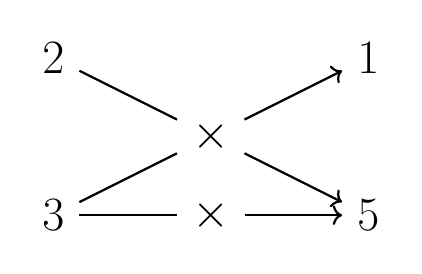
\begin{tikzpicture} 
\path ( 0, 0) node (times)   {$\times$};
\path (-2, 1) node (two)     {2};
\path ( 2, 1) node (one)     {1};
\path (-2,-1) node (three)   {3};
\path ( 2,-1) node (five)    {5};
\path ( 0,-1) node (timess)  {$\times$};
\draw [thick] (two) -- (times);
\draw [thick,->] (times) -- (five);
\draw [thick] (three) -- (times);
\draw [thick,->] (times) -- (one);
\draw [thick] (three) -- (timess);
\draw [thick,->] (timess) -- (five);
\end{tikzpicture}
\end{minipage}
\begin{minipage}[ht]{0.6\linewidth} \centering 
\begin{center}
\begin{align*}
&= \frac{(2 \times 5) + (3 \times 1)}{(3 \times 5)}\\\\
&= \frac{10+3}{15} = \frac{13}{15}
\end{align*}
\end{center}
\end{minipage}
\end{figure}

\begin{figure}[ht]
\begin{minipage}[ht]{0.4\linewidth} \centering
\begin{large}$\frac{3}{8}+\frac{2}{9}=$\end{large}\\
\vspace{8pt}
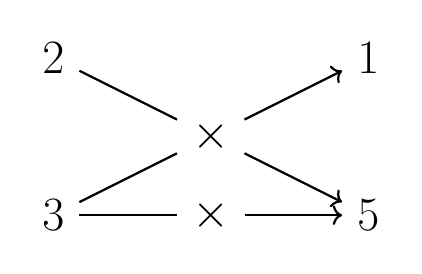
\begin{tikzpicture} 
\path ( 0, 0) node (times)   {$\times$};
\path (-2, 1) node (two)     {2};
\path ( 2, 1) node (one)     {1};
\path (-2,-1) node (three)   {3};
\path ( 2,-1) node (five)    {5};
\path ( 0,-1) node (timess)  {$\times$};
\draw [thick] (two) -- (times);
\draw [thick,->] (times) -- (five);
\draw [thick] (three) -- (times);
\draw [thick,->] (times) -- (one);
\draw [thick] (three) -- (timess);
\draw [thick,->] (timess) -- (five);
\end{tikzpicture}
\end{minipage}
\begin{minipage}[ht]{0.6\linewidth} \centering 
\begin{center}
\begin{align*}
&=\frac{(3\times9)+(8\times2)}{(8\times9)}\\
&=\frac{27+16}{72}=\frac{43}{72}.\\\\
\end{align*}
\end{center}
\end{minipage}
\end{figure}

\vspace{28pt}
\textbf{Congratulations! You can now add, subtract, multiply, and divide fractions just like you can do with whole numbers.}

\pagebreak

\section{Using prime numbers}
Here follows some extra methods you can use to find the lowest common denominator, for if you one day need to work out fractions with larger than usual numbers in them.

\subsection*{Using prime factor tallies\\to find the common denominator}
To find the lowest common denominator, multiply the largest count of each prime factor.\\

For example, $\frac{1}{4} + \frac{1}{5} + \frac{1}{12}$

Prime factors : $4 = 2 \times 2$, $5 = 5$, and $12 = 2 \times 2 \times 3$.

Tally of prime factors: 2: (2, 2), 3: (1), 5: (1).

Multiply the largest count of each prime factor: $2 \times 2 \times 3 \times 5 = 60$.

Divide the lowest common denominator (60) by the denominators to find the multiple needed to make the denominators equal, then multiply numerator and denominator of each fraction by that amount.
\begin{align*}
\frac{60}{4} &= 15 : &\frac{1}{4} \times \frac{15}{15} &= \frac{15}{60} \\
\frac{60}{5} &= 12 : &\frac{1}{5} \times \frac{12}{12} &= \frac{12}{60} \\
\frac{60}{12} &= 5 : &\frac{1}{12} \times \frac{5}{5} &= \frac{1}{60}
\end{align*}
Greatest common factor of $32$ and $60$ is $4$, so
$$\frac{15}{60} + \frac{12}{60} + \frac{5}{60} = \frac{32}{60}= \frac{^8\cancel{32}}{\cancel{60}_{15}} = \frac{8}{15}$$

\pagebreak

\subsection*{Cancelling common prime factors\\to find the common denominator}

\begin{doublespace}
Another way to find a common denominator is to list out the prime factors of the denominators and cancel any common factors. The lowest common denominator will be the product of the remaining prime factors.

For example, to find the common denominator of $8$ and $12$:

prime factors of $8$: $2 \times 2 \times 2$

prime factors of $12$: $2 \times 2 \times 3$

Note the common factors, cancel one of each pair, and multiply the rest: 
8 = \(\tikz[baseline=(math.base)]{\node[draw,circle,inner sep=1pt] (math) {\(\cancel{2} \times 2\)};} \times 2\), and 
12 = \(\tikz[baseline=(math.base)]{\node[draw,circle,inner sep=1pt] (math) {\(\cancel{2} \times 2\)};} \times 3\),

and $2 \times 2 \times 2 \times 3 = 24$.
\end{doublespace}

\pagebreak

\subsection*{Using powers of prime factors\\ to find the common denominator}


The lowest common denominator is the product of the highest powers of each prime factor.

For example, $$\frac{2}{540} + \frac{1}{72}$$

Denominators are 540 and 72. It’s easier to work out their prime factors than it is to multiply these large numbers. (Hint: do a prime factor tree.)
$$540 = 2 \times 2 \times 3 \times 3 \times 3 \times 5 \text{ and }72 = 2 \times 2 \times 2 \times 3 \times 3$$
Then write the factors as powers:
$$540 = 2^2 \times \boxed{3^3} \times \boxed{5^1}$$
$$72 = \boxed{2^3} \times 3^2$$

Pick out the prime factors with the highest powers and multiply them together to get the lowest common denominator.

$$2^3 \times 3^3 \times 5^1 = 8 \times 27 \times 5 = 1080$$

Now convert the fractions to both have the common denominator of 1080 by multiplying them appropriately:

$$\frac{2}{540} \times \frac{2}{2} = \frac{4}{1080}\text{ and }\frac{1}{72} \times \frac{15}{15} = \frac{15}{1080}$$
$$\text{so }\frac{2}{540} + \frac{1}{72} = \frac{4}{1080} + \frac{15}{1080} = \frac{19}{1080}$$

\vspace*{\fill}
\begin{center}
\linespread{2}\large

Enquiries

\textbf{Applied Scholastics Ferndale}

Principal: Paula McLennan

mobile phone: 0431 683 306

email address: apsferndale@gmail.com

website: apsferndale.webs.com
\end{center}
\vspace*{\fill}

\end{spacing}

\end{document}